\documentclass{article}
\usepackage{polski}
\usepackage[utf8]{inputenc}
\usepackage[top=3cm, bottom=3cm, left=3cm, right=3cm]{geometry}
\usepackage{secdot}
\sectiondot{subsection}
\usepackage{scrextend}
\usepackage{booktabs}
\usepackage{array}
\usepackage{ltablex}
\usepackage{amsmath}
\usepackage{amsfonts}
\usepackage{listings}
\usepackage{parskip}
\addtokomafont{labelinglabel}{\sffamily}
\usepackage{graphicx}
\graphicspath{ {./} }
\title{\vspace{7cm}\LARGE Analiza algorytmów\\semestr 16Z\\Projekt: Skąpa nauczycielka}
\author{\LargeŁukasz Wlazły\\nr albumu: 269365}
\date{}

\begin{document}
	\maketitle
	\pagenumbering{gobble}
	\newpage
	\pagenumbering{arabic}

	\section{Treść zadania}

	Nauczycielka w przedszkolu chce rozdać ciastka dzieciom w swojej grupie. Dzieci siedzą w linii obok siebie (i nie zmieniają pozycji). Każde dziecko ma przypisaną ocenę $  s_{i}, i \in (1, 2, \ldots, n) $ zgodnie z wynikiem testu umiejętności.
	Nauczycielka chce dac każdemu dziecko co najmniej jedno ciastko. Jeśli dzieci siedzą obok siebie, dziecko z wyższą oceną musi dostac więcej ciastek niż to z niższą oceną. Nauczycielka ma ograniczony budżet, więc chce rozdać jak najmniej ciastek. Zaproponuj algorytm, który zwróci najmniejszą liczbę ciastek, które musi rozdać nauczycielka.

	\section{Algorytm}

	\subsection{Założenia}

	Dane są ciągi $(s_{n})$ oraz $(r_{n})$, gdzie $n, \in \mathbb{N}$ oznacza liczbę dzieci, takie, że $s_{i}$ oznacza ocenę, a $s_{i}$ ilość ciastek $i$-tego dziecka.
	Lokalnym minimum nazywamy taką liczbę $l_m\in\mathbb{N}$, że:
	\begin{align*}
		i = l_m \Leftrightarrow
		\begin{cases}
			s_{i} < s_{i + 1}, & i = 1 \\
			s_{i-1} \leq s_{i} < s_{i+1}, & 1 < i < m
		\end{cases}
	\end{align*}

	Na początku ciąg $(s_{n})$ zawiera dane wejściowe, natomiast ciąg $(r_{n})$ jest wypełniony zerami. \\

	Przydział ciastek odbywa się zgodnie z zasadą:
	\begin{itemize}
		\item jeśli poruszamy się w kierunku rosnących wartości i, to:
			\begin{align*}
				r_i  =
				\begin{cases}
					r_{i-1}, & s_{i} = s_{i-1} \\
					r_{i-1} + 1, & s_{i} > s_{i-1} \\
					r_{i-1} - 1, & s_{i} < s_{i-1} \\
				\end{cases}
			\end{align*}

		\item jeśli poruszamy się w kierunku malejących wartości i, to:
			\begin{align*}
				r_i  =
				\begin{cases}
					max(r_{i+1}, r_{i}), & s_{i} = s_{i+1} \\
					max(r_{i+1} + 1, r_{i}), & s_{i} > s_{i+1} \\
					max(r_{i+1} - 1, r_{i}), & s_{i} < s_{i+1} \\
				\end{cases}
			\end{align*}
	\end{itemize}

	Wynikiem działania algorytmu jest ciąg $(r_{n})$, który spełnia następującą zasadę:
	\begin{align*}
		\forall_{i\in \{2, \ldots, n-1\}}\hspace{1em} (|r_i - r_{i+1}| = 1) \lor (|r_i - r_{i-1}| = 1)
	\end{align*}

	\newpage
	\subsection{Przebieg algorytmu}
	marks $\leftarrow$ dane wejściowe \\
	coockies $\leftarrow$ przydzielone ciastka

	\begin{lstlisting}[tabsize=2]
		coockies[1] := 1;

		for i := 2 to m:
			if i is local minimum:
				coockies[i] = 1
				continue

			if marks[i] > marks[i-1]:
				coockies[i] := coockies[i-1] + 1
			if marks[i] < marks[i-1]:
				coockies[i] := max(coockies[i-1] - 1, 1)
			if marks[i] = marks[i-1]:
				coockies[i] := coockies[i-1]

		for i := m-1 to 1:
			if i is local minimum:
				coockies[i] = 1
				continue

			if marks[i] > marks[i+1]:
				coockies[i] := max(coockies[i], coockies[i+1] + 1)
			if marks[i] < marks[i+1]:
				coockies[i] := max(coockies[i], max(coockies[i+1] - 1, 1))
			if marks[i] = marks[i-1]:
				coockies[i] := max(coockies[i], coockies[i+1])

		result := 0
		for i in coockies:
			result := result + i

		return result
	\end{lstlisting}

	\subsection{Złożoność pamięciowa}
	Przyjmując, że ocena jednego ucznia oraz ilość ciastek jaką dostaje zajmują jedną komórkę pamięci, algorytm posiada złożoność pamięciową określoną wzorem:
	\begin{align*}
		M(n) = 2n
	\end{align*}

	\subsection{Złożoność czasowa}
	Operacją podstawową algorytmu jest wykonanie obliczeń na pojedynczej komórce ciągu wejściowego lub pomocniczego. Wobec tego złożoność czasowa wynosi:
	\begin{align*}
		T(n) = 3n
	\end{align*}
	Zliczanie ciastek mogłoby zostać zoptymalizowane i włączone w dwie poprzednie pętle, jednak spowodowałoby to, że kod stałby się mniej czytelny.


	\section{Przypadki trywialne}

	\subsection{Ciąg stały}

	Jeśli wszystkie dzieci otrzymały taką samą ocenę, to wynikiem działania algorytmu jest:
	\begin{align*}
		n
	\end{align*}

	\subsection{Ciąg malejący lub rosnący}

	Jeśli oceny dzieci układają się w ciąg rosnący lub malejący, to wynikiem działania algorytmu jest:
	\begin{align*}
		\displaystyle\sum_{i=1}^{n} i
	\end{align*}

	\section{Testowanie algorytmu}

	\subsection{Maszyna}
	\begin{center}
		\begin{tabular}{c c}
			\toprule
			Procesor & Intel Core i5 6200U \\
			\midrule
			Pamięć & 8GB \\
			\midrule
			System Operacyjny & Arch Linux\\
			\bottomrule
		\end{tabular}
	\end{center}

	\subsection{Założenia teoretyczne}
	Złożoność obliczeniowa algorytmu implikuje wniosek, że n-krotny przyrost liczby dzieci powinien spodować n-krotny wzrost czasu rozwiązywania problemu. Testy zostaną przeprowadzone dla różnej liczby przypadków testowych oraz różnych wartości maksymalnej oceny, jaką mógł otrzymać uczeń.

	\subsection{Procedura testowania}
	W każdym przypadku zostało uruchomione 1000 testów. Maksymalna ocena, jaką mógł otrzymać uczeń było 400.
	Dla każdego testu liczba dzieci liczba dzieci jest losowana z przedziału [m - 5\%; m + 5\%].
	Wszystkie zestawy testów zostały wykonane jako procesy jednowątkowe.


	\subsection{Testy}

	\begin{center}
		\begin{tabular}{c c}
			\toprule
				Ilość dzieci & Średni czas [$\mu s$] \\
			\midrule
				100 & 21 \\
				1 000 & 101 \\
				10 000 & 784 \\
				100 000 & 7789 \\
				1 000 000 & 76235 \\
				8 000 000 & 612973 \\
			\bottomrule
		\end{tabular}

		\vspace{3cm}
		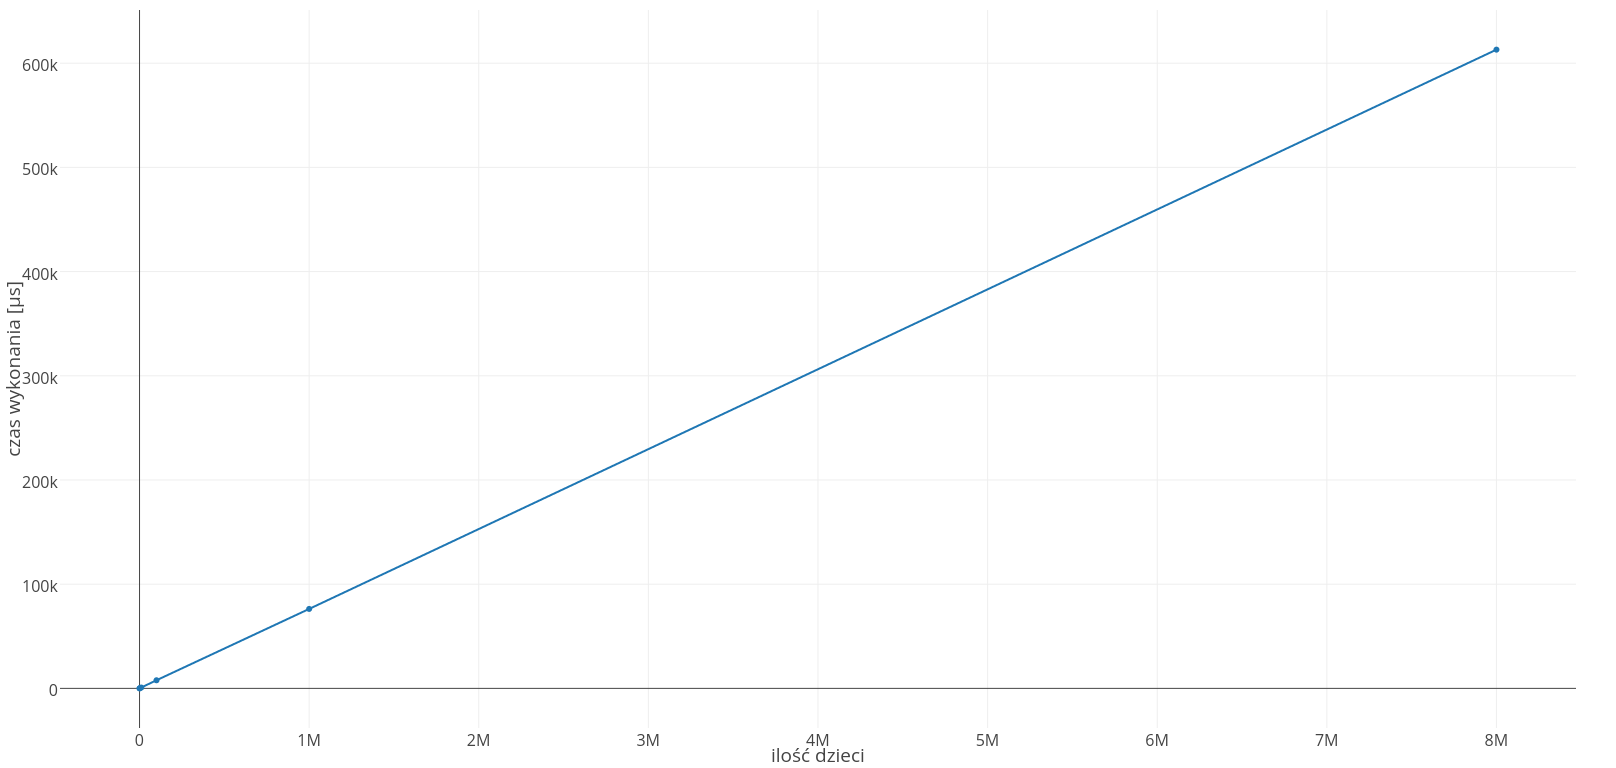
\includegraphics[width=\textwidth]{test_plot.png}
	\end{center}
\end{document}
